The simulator used for Hubo-Ach is the OpenHubo.
OpenHubo is an open-source kinematic and dynamic simulator for the the Hubo2 and Hubo2+ series robots.
It was developed by the Drexel Autonomous Systems Lab and runs using the open-source robot simulation environment OpenRAVE\cite{diankovThesis}.
Fig.~\ref{fig:openhubbo} shows the OpenHubo shell model and collision model.

\begin{figure}[thpb]
  \centering
      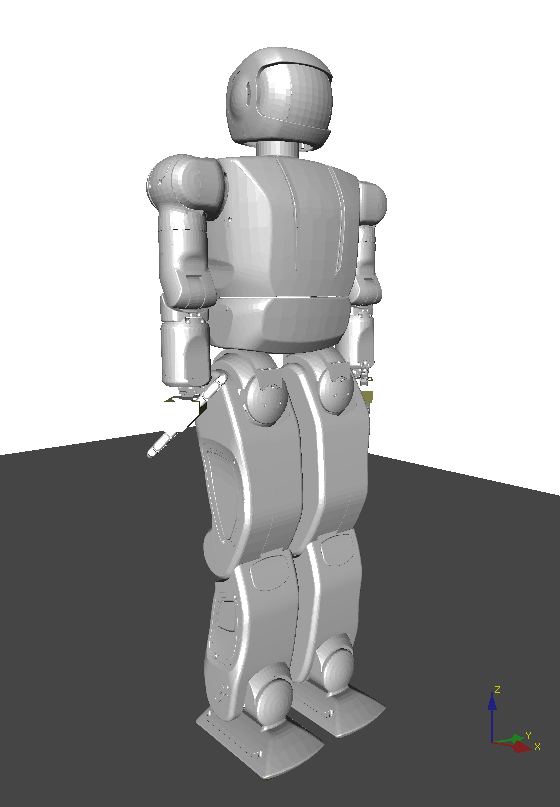
\includegraphics[width=0.4\columnwidth]{./pix/hBody.png}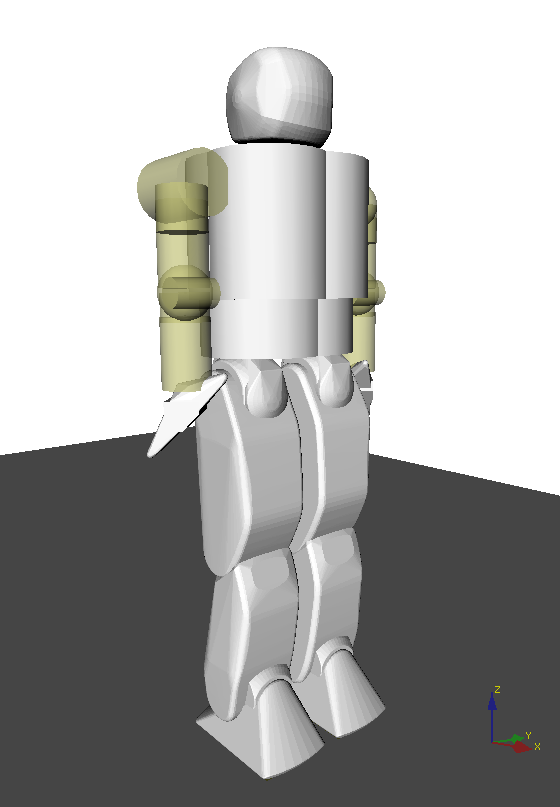
\includegraphics[width=0.4\columnwidth]{./pix/hCol.png}
      
\caption{OpenHubo model of the Hubo2 humanoid robot developed by the Drexel Autonomous Systems Lab and runs using the open-source robot simulation environment OpenRAVE\cite{diankovThesis}.  (Left) Shell Model - High polygon count.  (Right) Collision model - Made with primitives.}
\label{fig:openhubbo}
\end{figure}

The masses and lengths are of the OpenHubo model are all based off of the CAD model.
The shell model includes an external skin based off of the CAD model of the Hubo's shell.
This model is high polygon count and thus tends to require more processing time to detect collisions.
The collision model is constructed out of primitives in order to decrease the complexity of the model and decrease required processing time.
The collision model is a representation of the shell model. 
It does not precisely fit the contours but through experimentation and use has been calibrated to be a good representation of the Hubo's outer shell.

Fig~\ref{fig:openhubosim} shows the diagram of how the OpenHubo simulator is connected to Hubo-Ach.  
No changes to previous controllers are required for them to work with the simulator.
Just as before the desired reference $\theta_d$ being filtered before applied to Hubo via Hubo-Ach.  
$\theta_d$ is sent through a filter that reduces the \textit{jerk} on the actuator then the new reference $\theta_r$ is set on the \textbf{FeedForward} channel, Hubo-Ach reads it then commands Hubo at the rising edge of the next cycle.  
At this point the \textit{to simulator} trigger, $\Gamma_{ts}$, is set high and the OpenHubo simulator reads $\theta_c$.
The simulator waits until Hubo-Ach is ready until it starts its next set of cycles.
The reference is set within OpenHubo and solved with a simulation period of $T_{sim}$.
The simulation period $T_{sim}$ must be an integer deviser of the robot real-time period $T_r$.
In this case

\begin{equation}
T_r=0.005~s
\end{equation}

\begin{equation}
T_{sim} = \frac{T_r}{n}
\end{equation}


Once the simulator has gone through $n$ cycles the current state, $H_{state}$ is placed on the Hubo-Ach \textbf{FeedForward} channel and the ready trigger $\Gamma_{fs}$ is raised.  
Hubo-Ach is waiting for the rising edge of the \textit{from simulator} trigger, $\Gamma_{fs}$, to continue on to the next cycle.

\begin{figure}
\centering

\begin{tikzpicture}[->,>=stealth',shorten >=1pt,auto,node distance=5cm,
  thick,main node/.style={fill=white!20,draw,font=\sffamily\Large\bfseries}]


  \node[main node] (ctrl) {Controller};
  \node[main node] (filter) [right=1.5cm of ctrl] {Filter};
  \node[main node] (hubo-ach) [below=1.0cm of filter] {Hubo-Ach};
  
  \node[main node,font=\small] (hold1) [right=1.5cm of hubo-ach, yshift=0.5cm] {hold};
  \node[main node,font=\small] (hold2) [right=1.5cm of hubo-ach, yshift=-0.5cm] {hold};

  \node[main node] (hubo) [right=1.5cm of hold1, yshift=-0.5cm] {OpenHubo};




%  \path[->, every node/.style={font=\sffamily\small}]
%    (hubo-ach) edge node [above] {$\theta_c$} (hubo);

\draw[->] ([yshift=0.2 cm]hubo-ach.east)  to [out=0,in=-180] node [below] {$\theta_c$} ([yshift=-0.0 cm]hold1.west)  ;
\draw[->] ([yshift=0.0 cm]hold1.east)  to [out=0,in=-180] node [below] {$\theta_c$} ([yshift=0.2 cm]hubo.west)  ;
\draw[-*] ([xshift=1.0 cm]hubo-ach.north)  to [out=60,in=120] node [above] {$\Gamma_{ts}$} ([yshift=-0.05 cm]hold1.north)  ;



\draw[->] ([yshift=0.0 cm]hold2.west)  to [out=180,in=0] node [below] {$H_{state}$} ([yshift=-0.2 cm]hubo-ach.east)  ;
\draw[->] ([yshift=-0.2 cm]hubo.west)  to [out=180,in=0] node [below right] {$H_{state}$} ([yshift=0.0 cm]hold2.east)  ;
\draw[-*] ([xshift=0.0 cm]hubo.south)  to [out=-120,in=-60] node [above] {$\Gamma_{fs}$} ([yshift=0.05 cm]hold2.south)  ;

\draw[->] ([yshift=-0.0 cm]hubo-ach.west)  to [out=180,in=-90] node [below left] {$H_{state}$} ([yshift=0.0 cm]ctrl.south)  ;



%\draw[->] ([yshift=-0.2 cm]hubo.west)  -- node [below] {$H_{state}$} ([yshift=-0.2 cm]hubo-ach.east)  ;
%\draw[->] ([yshift=-0.0 cm]hubo.south)  to [out=-120,in=-60] node [below] {$\Gamma_{fs}$} ([yshift=-0.0 cm]hubo-ach.south)  ;



  \path[->,every node/.style={font=\sffamily\small}]
    (ctrl) edge node [above] {$\theta_d$} (filter);

 \draw[->] ([xshift=-0.5 cm]filter.south)  -- node [left] {$\theta_r$} ([xshift=-0.5 cm]hubo-ach.north)  ;
 \draw[->] ([xshift=0.5 cm]hubo-ach.north) -- node [left] {$\theta_a$} ([xshift=0.5 cm]filter.south)  ;


\end{tikzpicture}
\caption{Desired reference $\theta_d$ being filtered before applied to Hubo via Hubo-Ach.  $\theta_d$ is sent through a filter that reduces the \textit{jerk} on the actuator then the new reference $\theta_r$ is set on the \textbf{FeedForward} channel, Hubo-Ach reads it then commands Hubo at the rising edge of the next cycle.}
\label{fig:hubo-ach-feedforwardFilter}
\end{figure}




The external controllers do not know weather Hubo-Ach is running in \textit{simulation} or \textit{real-time} mode.  
In order to ensure a Hubo-Ach controller stays what ever timing method is being used the controller can do any of the following:

\begin{itemize}
\item Wait for the $\Gamma_{fs}$ trigger
\item Wait for a new $H_P{state}$ to be updated
\item Watch the time listed within $H_{state}$
\end{itemize}

If the given task does not require physics or feedback from $H_{state}$ then you can run in \textit{no physics} mode.
\textit{No physics} mode only gives collisions, joint angles and ideal feedback from the sensors.
In addition \textit{no physics} is capable of running much faster then real-time if needed.



\begin{table}
\centering
\caption{OpenHubo simulator sim-time and real-time comparison chart.  Shows the maximum percent real-time the OpenHubo simulator is capable of preforming at where 100\% is real-time.  All tests were preformed on an Intel i7 running at 2.8Ghz with 18Gb of RAM.}
\begin{tabular}{| l || c | c |}
\hline
Mode               & Timing                & Maximum Percent Real-Time (\%) \\
\hline
\hline
Physics            & Sim-Time              & 37\%   \\
\hline
No Physics         & Real-Time or Sim-Time & 362\%  \\
\hline
\end{tabular}\label{table:simtime}
\end{table}


Fig.~\ref{fig:huboOpenHuboWalking} shows the capability of Hubo-Ach to run in both sim-time and real-time modes.  
This is the same statically stable trajectory as seen in Section~\ref{sec:WalkingPatternGeneration}


\begin{figure}[thpb]
  \centering
      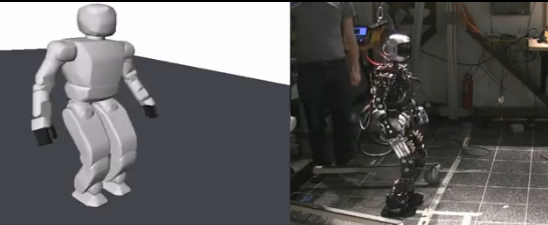
\includegraphics[width=0.69\columnwidth]{./pix/huboandopenhubowalking.png}
      
\includegraphics[width=0.3\columnwidth]{./qrcode/qrcode-hubo-openhubo-walking.png}\\
      Video: http://danlofaro.com/phd/walking/\#WalkingHuboAndOpenHubo
\caption{Hubo and OpenHubo walking using Hubo-Ach in Real-Time and Sim-Time Respectively}
\label{fig:huboOpenHuboWalking}
\end{figure}

